\section{Afbakening}
%
% wat wil ik zeggen 
% - Het huidige Snakware cloud platform is erg groot en kunnen nooit alles maken dat het platform klan
% - Het huidige platform bestaat uit 3 verschillende applicaties: CMS-API, de Snakeware cloud frontend , de klant zijn web applicatie.
% - wat er wordt gemaakt is de de CMS-API en de klant zijn webapplicatie te de content tonen
%
Het huidige Snakware cloud plaform heeft in de loop der jaren veel functionaliteiten gekregen.
Hierom is het van belang dat tijdens de afstudeerperiode de opdracht niet te groot wordt gemaakt om het succesvol te kunnen afronden.
Daarom wordt er primair gefocust op het realiseren en ontwerpen van de CMS-API.

\whitespace[2]
Snakeware cloud bestaat momenteel uit 3 verschillende applicaties, deze applicaties zijn:
\begin{itemize}
    \item[-] Snakeware cloud \gls{GUI}  
    \item[-] CMS-API
    \item[-] klant webapplicatie
\end{itemize}

\whitespace[2]
Er is besloten om niet de Snakeware cloud \gls{GUI} te maken om de scope van de afstudeeropdracht haalbaar te maken.
Daarnaast wordt de klant webapplicatie minimaal uitgewerkt om de data van de CMS-API te kunnen tonen.
Om de \gls{UserJourneys} te kunnen valideren worden ze getest door middel van postman workflows.
Voor verheldering is in figuur \ref{fig:ProductOverview} een versimpelde communicate diagram van de producten die gemaakt en niet gemaakt worden tijdens de afstudeer opdracht.\\
\begin{graphic}
    \vspace{0.2cm}
    \captionsetup{type=figure}
    \caption{Gesimplificeerde communicatie diagram van  systemen}
    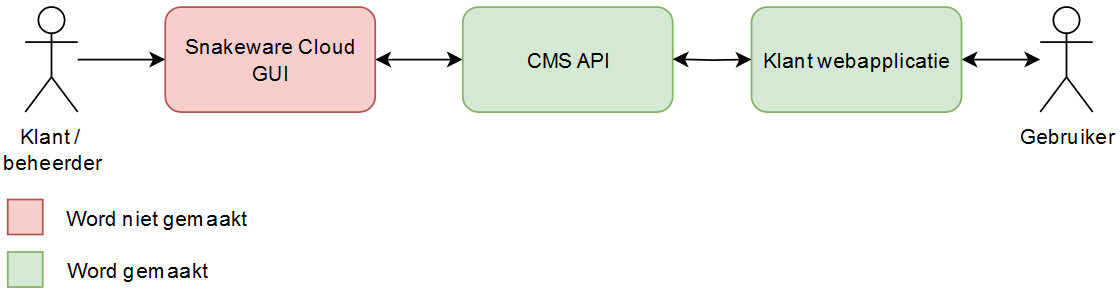
\includegraphics[scale=0.4]{ProductCommunicate}
    \label{fig:ProductOverview}
    \vspace{0.2cm}
\end{graphic}
